% vim: set textwidth=78 autoindent:

\subsection{Decorations Plugins}

% when the revision of a section has been finalized, 
% comment out the following line:
% \updatedisclaimer

The Decorations Plugins includes the Copyright Label Plugin, the North 
Arrow Plugin and the Scale Bar Plugin. They are used to ``decorate'' the 
map by adding cartographic elements. 

\subsubsection{Copyright Label Plugin}

The title of this plugin is a bit misleading - you can add any random text to the map.

\begin{figure}[ht]
   \begin{center}
   \caption{Copyright Label Plugin \nixcaption}\label{fig:copyright}\smallskip
   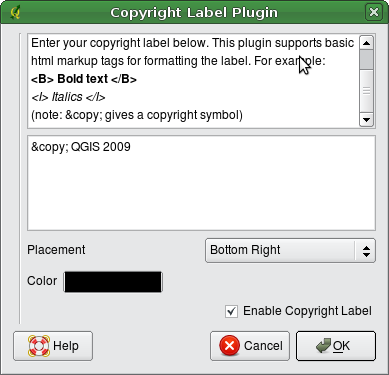
\includegraphics[clip=true, width=8cm]{copyright}
\end{center}  
\end{figure}

\begin{enumerate}
\item Make sure the plugin is loaded
\item Click on \mainmenuopt{Plugins} > \dropmenuopt{Decorations} > \dropmenuopttwo{copyright_label}{Copyright Label} or use the \toolbtntwo{copyright_label}{Copyright Label} button from the Toolbar.
\item Enter the text you want to place on the map. You can use HTML as
  shown in the example
\item Choose the placement of the label from the \selectstring{Placement}{Bottom Right} drop-down box
\item Make sure the \checkbox{Enable Copyright Label} checkbox is checked
\item Click \button{OK} 
\end{enumerate}

In the example above (default) places a copyright symbol followed by the date in the 
lower right hand corner of the map canvas.

\subsubsection{North Arrow Plugin}

The North Arrow plugin places a simple north arrow on the map canvas. At
present there is only one style available. You can adjust the angle of the
arrow or let QGIS set the direction automatically. If you choose to let
QGIS determine the direction, it makes its best guess as to how the arrow
should be oriented. For placement of the arrow you have four options, 
corresponding to the four corners of the map canvas.

\begin{figure}[ht]
   \begin{center}
   \caption{North Arrow Plugin \nixcaption}\label{fig:north_arrow}\smallskip
   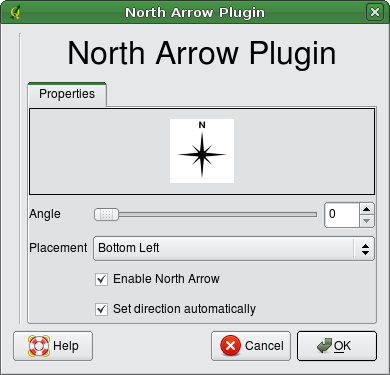
\includegraphics[clip=true, width=8cm]{north_arrow_dialog}
\end{center}  
\end{figure}

\subsubsection{Scale Bar Plugin}
The Scale Bar plugin adds a simple scale bar to the map canvas. You
control the style and placement, as well as the labeling of the bar. 

QGIS only supports displaying the scale in the same units as your map frame. So
if the units of your layers are in meters, you can't create a scale bar in
feet. Likewise if you are using decimal degrees, you can't create a scale
bar to display distance in meters.

To add a scale bar:

\begin{enumerate}
\item Click on \mainmenuopt{Plugins} > \dropmenuopt{Decorations} > \dropmenuopttwo{scale_bar}{Scale Bar} or use the \toolbtntwo{scale_bar}{Scale Bar} button from the Toolbar.
\item Choose the placement from the \selectstring{Placement}{Bottom Left} drop-down list
\item Choose the style from the \selectstring{Scale bar style}{Tick Down} list
\item Select the color for the bar \selectcolor{Color of bar}{black} or use the default black color
\item Set the size of the bar and its label \selectnumber{Size of bar}{30 degrees}
\item Make sure the \checkbox{Enable scale bar} checkbox is checked
\item Optionally choose to automatically snap to a round number when the
  canvas is resized \checkbox{Automatically snap to round number on resize}
\item Click \button{OK} 
\end{enumerate} 

\begin{figure}[ht]
   \begin{center}
   \caption{Scale Bar Plugin \nixcaption}\label{fig:scale_bar}\smallskip
   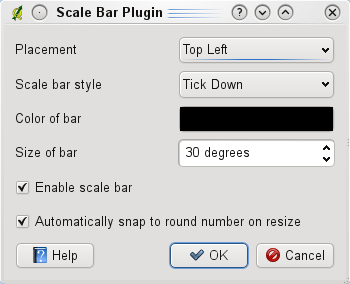
\includegraphics[clip=true, width=8cm]{scale_bar_dialog}
\end{center}  
\end{figure}

\begin{Tip}\caption{\textsc{Plugins Settings Saved to Project}}\index{plugins settings}
\qgistip{When you save a .qgs project, any changes you have made to NorthArrow, ScaleBar and Copyright plugins will be saved in the project and restored nexttime you load the project.}
\end{Tip}

